\section{Approach}

Algorithm \ref{algo:core-exp} summarizes the main steps of our approach.
In this section we present these steps in detail, and give an end-to-end example.

As seen in the pseudocode, the approach takes as input a \emph{pattern} $p$, besides
the thematic dictionary and the regular dictionary.
A {pattern} is a rectangular grid of a given size, with zero or more black cells and no letters.

\begin{figure}
\centering
\begin{tabular}{ccc}
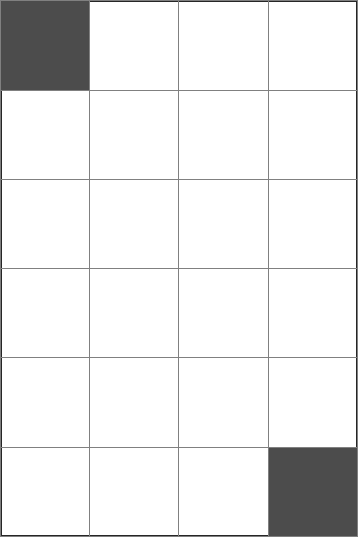
\includegraphics[width=.15\textwidth]{_plots/6x4-puzzle.pdf} & &
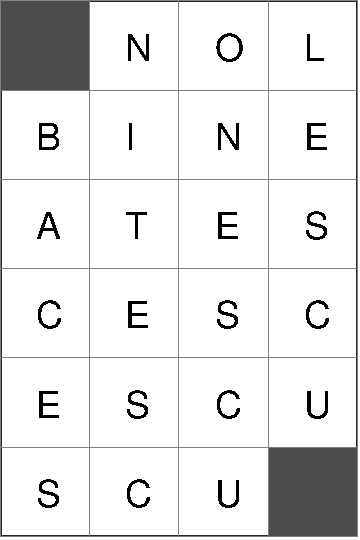
\includegraphics[width=.15\textwidth]{_plots/core-6x4-puzzle.pdf}
\end{tabular}
\caption{Left: A pattern defined as a $6 \times 4$ grid with two black cells, in the top-left corner and the bottom-right corner. Right: A core based on the pattern at hand.}
\label{fig:pattern}
\end{figure}

Figure \ref{fig:pattern} (left) shows an example of a pattern. It is a $6 \times 4$ grid with two black cells, one in the top-left corner and one in the bottom-right corner.
Observe that the pattern is significantly smaller than the $13 \times 13$ size of the full-size grid.
The pattern will end up being integrated inside the full-size solutions generated with our approach,
as we will show in this section.

\begin{algorithm}[t]
\DontPrintSemicolon % Some LaTeX compilers require you to use \dontprintsemicolon instead
\KwIn{Pattern $p$, thematic dictionary and regular dictionary}
%\KwOut{Full solutions}
%\tcc{Search for a full solution}
$C \leftarrow \mbox{GenerateCores}(p)$\;
$E \leftarrow \mbox{ExpandCores}(C)$\;
$S \leftarrow \mbox{GenerateSeeds}(E)$\;
Rank $S$ and put top $k$ elements into a list $S'$\;
\For{$s \in S'$} {
    $\mbox{Evolve}(s)$\;
}
\caption{{\sc Generating full solutions.}}
\label{algo:core-exp}
\end{algorithm}


\subsection{Generating Cores}

Step 1 in Algorithm \ref{algo:core-exp} generates a collection of so-called \emph{cores} from the pattern $p$.
A core is a pattern filled with letters on the white cells.
We require that, in a full solution returned with Algorithm \ref{algo:core-exp}, 
the sub-area corresponding to the pattern will have a perfect score.
In other words, each white cell in the pattern will contribute two points.

To achieve this, we construct and solve a small crosswords puzzle instance.
The grid is the pattern $p$. There is only one dictionary, which contains 
substrings of the thematic words.
It is sufficient to consider only substrings of the lengths that 
correspond to the lengths of the word slots in the pattern.

In our running example, word slot lengths are 3, 4, 5, and 6.
For example, when generating substrings of length 4,
if IONESCU and POPESCU are thematic words,
the substrings generated are IONE, ONES, NESC, ESCU, POPE, OPES, PESC, and ESCU.
Duplicates such as ESCU are kept only once.

The small crosswords puzzle instance constructed in this way is 
solved with the {\sc Wombat} solver.
The solver enumerates all solutions, which are precisely the 
cores computed at step 1 in Algorithm \ref{algo:core-exp}.
Figure \ref{fig:pattern} (right) shows an example of a core.



\subsection{Expanding Cores}

\begin{figure}
\centering
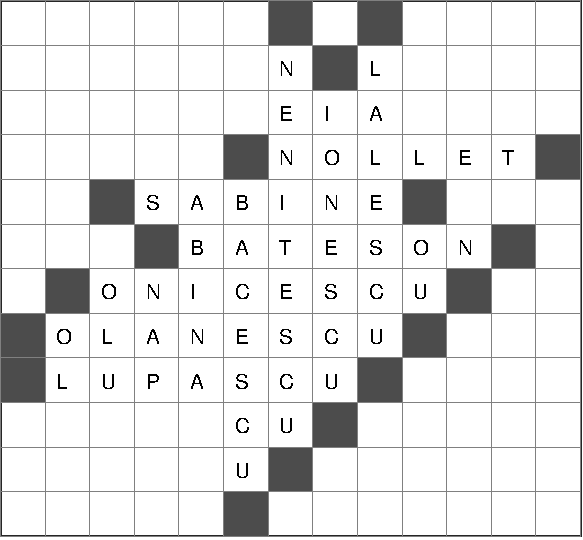
\includegraphics[width=.45\textwidth]{_plots/extcore-alive-0-puzzle-72-2975-1488--1--1.pdf}
\caption{An expanded core based on the core shown in Figure \ref{fig:pattern} (right).}
\label{fig:exp-core}
\end{figure}


At step 2, each core is expanded by placing full thematic words on top of the substrings present in the core at hand.
For each thematic word added to an expanded core, we add two black cells at its corresponding endpoints.
Figure \ref{fig:exp-core} shows an example of an expanded core. 
The cells on the top row, bottom row, leftmost column and rightmost column form the \emph{border} of the expanded core. The rest of the cells are the \emph{inner part} of the expanded core.
We define the \emph{inner size} as $h \times w$, where $h$ is the number of rows
of the inner part and $w$ is the number of columns.
In Figure \ref{fig:exp-core}, the inner size is $10 \times 11$.
Observe that the border can only contain black cells and empty cells.
The inner part can contain letters, black cells and empty cells.

As shown later in this section, the inner part of an extended core will be fit inside a full solution.
All or part of the border may or may not be included in a full solution, as explained later on.

More than one expanded core can exist for a given core (e.g., a substring such as ESCU can be expanded into multiple thematic words, such as IONESCU and POPESCU).
We generate expanded cores with a depth-first search.

We say that an extended core is a deadend (or, equivalently, it is dead) if no full valid solution can contain the extended core at hand. We label an extended core as dead, and filter it away, if any of the
following conditions is met:
it contains a word repetition; it contains a sequence of letters that cannot
possibly be expanded into a full word; or it contains adjacent black cells within the inner part.
Note that, at this stage, we don't check for adjacent black cells on the border.
Such a test will be performed later, after it is decided which part of the
border, if any, will be kept in a full-size solution, as shown later in this section.


\subsection{Generating Seeds}

\begin{figure*}
\centering
\begin{tabular}{ccc}
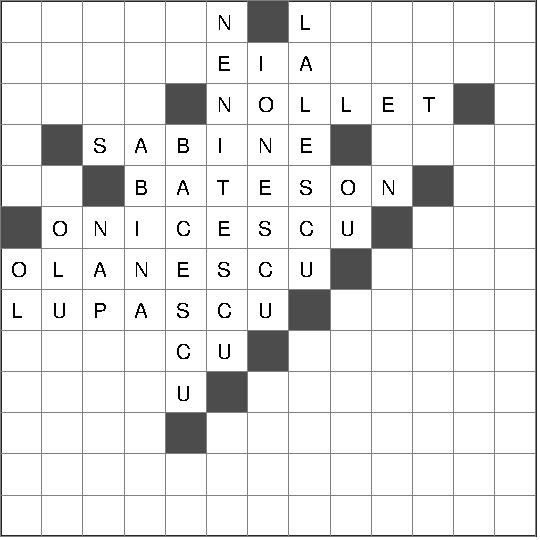
\includegraphics[width=.32\textwidth]{_plots/alive-0-puzzle-72-2975-1488--1--1.pdf} &
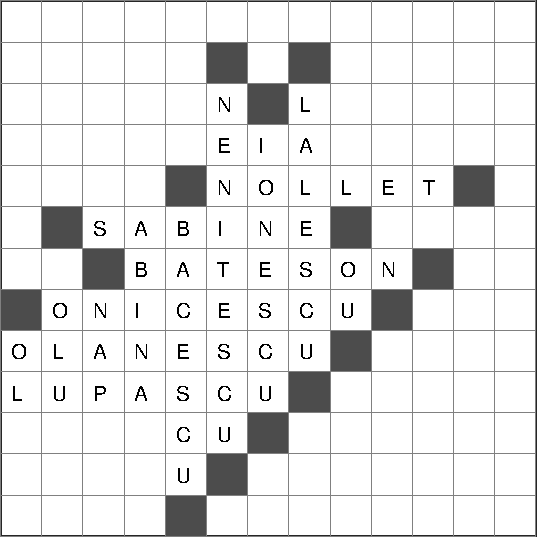
\includegraphics[width=.32\textwidth]{_plots/alive-0-puzzle-72-2975-1488--1-1.pdf} & 
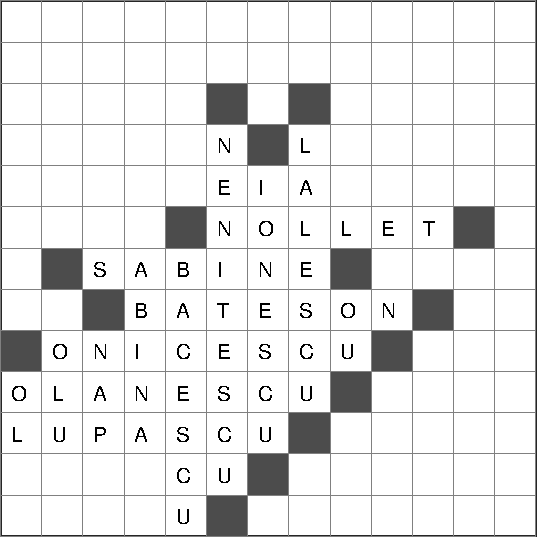
\includegraphics[width=.32\textwidth]{_plots/alive-0-puzzle-72-2975-1488--1-2.pdf}
\end{tabular}
\caption{A few seeds generated from the extended core shown in Figure \ref{fig:exp-core}.}
\label{fig:seeds}
\end{figure*}

When the inner size of an extended core $e$ is $13 \times 13$, it fits inside a full $13 \times 13$ grid in a unique way. However,
if the inner height and/or width are smaller than 13, $e$ can fit inside a full grid in multiple positions,
obtained by shifting it inside the full grid vertically and/or horizontally.

Each fitting of an extended seed inside a full grid is called a \emph{seed}.
As such, a seed is a full-size $13 \times 13$ grid, with 
letters, black cells and empty cells.
Figure \ref{fig:seeds} shows a few seeds generated from an extended core.

When the first column of the inner part of $e$ coincides 
with the first column of the seed, the leftmost column of $e$'s border
is left out from the seed. 
Otherwise, it is kept within the seed.
Other parts of the border (top row, bottom row, rightmost column)
are left out or kept inside in a similar way.
For example, in Figure \ref{fig:seeds} (left), the leftmost border column 
and the top border row are left out.
The seed in Figure \ref{fig:seeds} (middle) leaves out the
leftmost border column.
The seed at the right of Figure \ref{fig:seeds} leaves out
the leftmost border column and the bottom border row.


A seed is post processed with two objectives: to detect dead seeds 
(e.g., seeds that cannot be possibly expanded into a valid full solution); 
and, for seeds that are still alive, to detect, if possible, 
forced black cells and forced letters can could be added to the seed.
Given a position (cell) in a seed,
we say that a black cell or a letter is forced onto a 
given position if 
every possible full solution based on that seed must contain 
the black cell or letter at hand on the corresponding position.

Algorithm \ref{algo:fixpoint} shows seed post-processing in pseudocode.
Deadend detection includes checking for closures and semi-closures;
adjacent black cells\footnote{As this test is applied to the full
grid, it covers the part of the extended seed border, if any, that was
kept in the seed.}; 
word repetitions; and
sequences of letters that do not match with any word from the dictionaries.

Forced black cells are detected when all dictionary words matching 
a given sequence of letters in the seed would start in the same cell,
forcing the placement of a black cell on the cell before.
Similarly, forced black cells can be detected when 
all matching words finish on the same cell, forcing a black cell 
on the cell after.
Forced letters are detected when all matching words have the same 
letter on a given position.


\begin{algorithm}[t]
\DontPrintSemicolon % Some LaTeX compilers require you to use \dontprintsemicolon instead
\KwIn{Seed $s$ labelled alive}
%\KwOut{Full solutions}
%\tcc{Search for a full solution}
\Repeat{ until reaching fixpoint} {
    \If {deadend detected} {
        Label $s$ as dead\;
        Break\;
    }
    Add forced moves (black cells and words) to $s$\;
}
\Return $s$ and label (dead/alive)
\caption{{\sc Fixpoint computation.}}
\label{algo:fixpoint}
\end{algorithm}

\subsection{Ranking Seeds}

VADIM

\subsection{Evolving Seeds}

VADIM